\section{Issues Encountered So Far}

\subsection*{Non-Deterministic Nature of the Extraction Algorithm}

The extraction algorithm used by RA is non-deterministic,
meaning that for the same input code, the output of the extraction process can
vary. This results in different versions of semantically equivalent but
syntactically distinct code. In other words, while the extracted code maintains
the same functionality, its structure and readability can change between runs.
This poses a significant challenge for testing the tool, as each run may yield
different outputs for the same input, making consistent verification difficult. \\
For example in Figure \ref{fig:issue1}, a test of function extraction, RA may choose to pass
variables by reference to the extracted function, dereferencing them inside the
function body. In another instance, it might pass the same variables by
ownership, altering the code's appearance but not its behavior. While both
versions of the code will likely compile to identical machine code, the
readability and clarity of the resulting code can vary.

\begin{figure}[H]
    \centering
    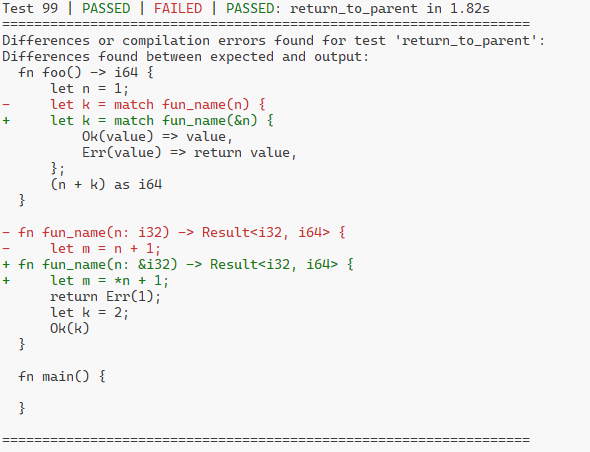
\includegraphics[width=\columnwidth]{Figures/issue_1.png}
    \caption{An example of the non-deterministic nature of the extraction
    algorithm. \textcolor{red}{Red is expected output}, \textcolor{green}{green is the
    returned code}}
    \label{fig:issue1}
\end{figure}

\subsection*{Come up with something else to go here}